\documentclass[11pt,a4paper,onecolumn]{exam}
\usepackage{amsmath}
\usepackage{amsthm}
\usepackage{amssymb}
\usepackage{graphicx}
\usepackage{float}
\usepackage[top=0.75in, bottom=0.75in, left=0.5in, right=0.5in]{geometry}
\usepackage{tikz}
\usepackage[skins]{tcolorbox}
\usepackage{listings}
\usepackage{xcolor}
\usepackage{hyperref}
\usepackage{multirow}
\usepackage{adjustbox}
\usepackage{booktabs}
\usepackage[font=small]{caption}
\usepackage{subcaption}

\definecolor{codegreen}{rgb}{0,0.6,0}
\definecolor{codegray}{rgb}{0.5,0.5,0.5}
\definecolor{codepurple}{rgb}{0.58,0,0.82}
\definecolor{backcolour}{rgb}{0.95,0.95,0.92}

\lstdefinestyle{mystyle}{
    backgroundcolor=\color{backcolour},
    commentstyle=\color{codegreen},
    keywordstyle=\color{magenta},
    numberstyle=\tiny\color{codegray},
    stringstyle=\color{codepurple},
    basicstyle=\ttfamily\footnotesize,
    breaklines=true,
    captionpos=b,
    keepspaces=true,
    numbers=left,
    numbersep=2pt,
    showspaces=false,
    showstringspaces=false,
    showtabs=false,
    tabsize=1
}

\newcommand{\questionheader}[1]{%
  \begin{tcolorbox}[
    enhanced,
    colback=black,
    coltext=white,
    boxrule=0pt,
    fontupper=\Large\bfseries,
    arc=4mm
  ]
  #1
  \end{tcolorbox}%
}

\lstset{style=mystyle, language=Python}

\begin{document}

\begingroup
    \centering
    \LARGE E1 213 Pattern Recognition and Neural Network\\
    \LARGE Assignment 2\\[0.5em]
    \large Dwaipayan Haldar\par
    \large \today\\[0.5em]
\endgroup
\noindent\rule{\textwidth}{0.5pt}
\printanswers
\renewcommand{\solutiontitle}{\noindent\textbf{Ans:}\enspace}


\questionheader{Phase 1: The MLP Baseline \& Gradient Flow (Air Quality)}

\textbf{1.1 Flattened Temporal MLP (Regression)}
\begin{solution}
A 3-layer MLP is trained on 72-hour flattened feature vectors to predict $t{+}24$ PM2.5. The data is split chronologically (70/15/15) with train-split normalization to prevent leakage. Test MSE (normalized) = \textbf{0.8568}.
\end{solution}

\textbf{1.2 The Vanishing Gradient Proof}
\begin{solution}
The sigmoid activation $\sigma(x)$ has derivative $\sigma'(x) = \sigma(x)(1{-}\sigma(x)) \leq 0.25$. Backpropagation multiplies these derivatives across layers, so the gradient of layer 1 scales as $(0.25)^3 \approx 0.016$ relative to the output layer. Fig.~\ref{fig:1_2} confirms this: the $L_2$ gradient norm of the first layer is orders of magnitude smaller than the third.
\end{solution}

\textbf{1.3 Imbalanced Threshold Classification}
\begin{solution}
PM2.5 $> 200$ is labelled hazardous (class 1). Standard BCE gives recall of 61\% for the minority class, while Weighted BCE (pos\_weight $\approx$ 2.86) improves minority recall to 78\% at the cost of some precision for a threshold of 0.5. Interesting thing is that the PR curve looks almost similar. That is because the training and testing has very different demographic. The testing has much more PM2.5 $> 200$ cases than the train one.
\end{solution}

\begin{figure}[H]
\centering
\begin{subfigure}[b]{0.50\textwidth}
    \centering
    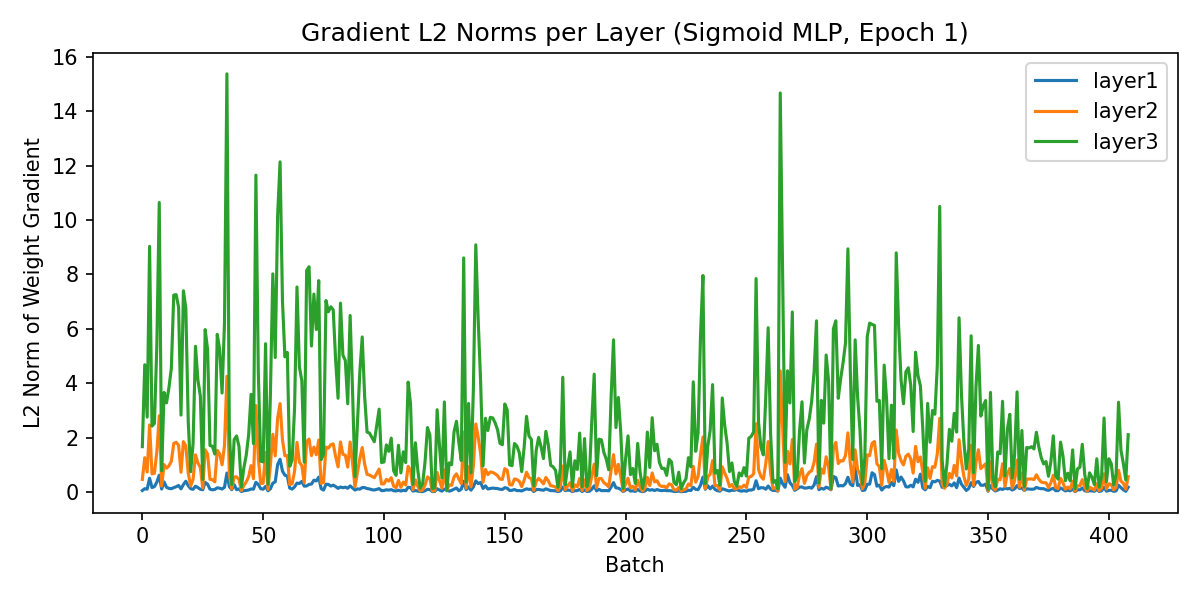
\includegraphics[width=\textwidth]{gradient_flow_sigmoid.png}
    \caption{$L_2$ gradient norm per layer (Sigmoid MLP, Epoch 1)}
    \label{fig:1_2}
\end{subfigure}
\hfill
\begin{subfigure}[b]{0.46\textwidth}
    \centering
    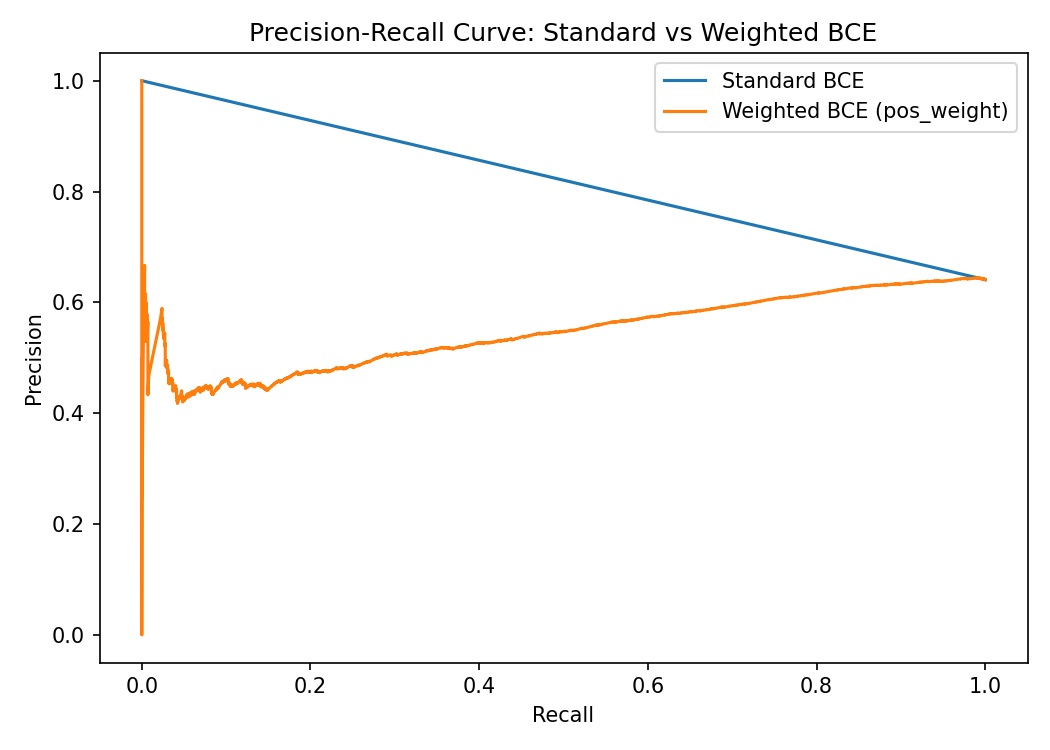
\includegraphics[width=\textwidth]{pr_curve_1_3.png}
    \caption{Precision-Recall: Standard vs.\ Weighted BCE}
    \label{fig:1_3}
\end{subfigure}
\end{figure}

\questionheader{Phase 2: CNNs \& Spatial Hierarchies (PlantVillage)}

\textbf{2.4 CNN from Scratch \& Receptive Fields}
\begin{solution}
The CNN has three Conv-BN-MaxPool blocks (8, 16, 32 filters) followed by three linear layers. Tensor shapes for a $128\times128$ input: $(1,3,128,128)\!\to\!(1,8,128,128)\!\to\!(1,8,64,64)\!\to\!(1,16,64,64)\!\to\!(1,16,32,32)\!\to\!(1,32,32,32)\!\to\!(1,32,16,16)\!\to\!(1,8192)\!\to\!(1,256)\!\to\!(1,38)$. The theoretical receptive field of a final feature-map activation is \textbf{22 pixels}, computed as $\text{RF}_n = \text{RF}_{n-1} + (k-1)\prod_{i<n}s_i$ iterated over the three conv+pool stages.
\end{solution}

\textbf{2.5 CNN Regression Head}
\begin{solution}
The classification head is replaced with a single linear output and MSE loss. The severity target is synthesized as the bounding-box ratio of necrotic pixels to total leaf area. Test MAE = \textbf{0.2392}.
\end{solution}

\textbf{2.6 Translation Invariance}
\begin{solution}
Baseline accuracy on 100 test images: \textbf{86.00\%}. After a 5-pixel shift: \textbf{77.00\%} — a drop of 9\%. Max-pooling provides only local invariance within each $2\times2$ window. A 5-pixel shift moves features across pooling-cell boundaries, changing which neuron ``wins,'' so the downstream representation changes and exact translation invariance is not achieved.
\end{solution}

\questionheader{Phase 3: RNNs \& Sequential Memory (Air Quality)}

\textbf{3.7 Vanilla RNN from Scratch}
\begin{solution}
A single-layer RNN is built using \verb|nn.Linear| layers and a \verb|tanh| loop: $h_t = \tanh(W_{hh}h_{t-1} + W_{xh}x_t + b)$. Trained with Adam ($\text{lr}=10^{-3}$, hidden=64) for 100 epochs with early stopping. Test MSE (normalized) = \textbf{0.9198}.
\end{solution}

\textbf{3.8 BPTT Decay}
\begin{solution}
Gradient magnitudes extracted via \verb|retain_grad()| on CPU: $\|\partial L/\partial h_{100}\| = 1.79\times10^{-1}$, $\|\partial L/\partial h_{50}\| \approx 0$, $\|\partial L/\partial h_0\| \approx 0$. The gradient scales as $\|W_{hh}^\top\|^{T-t}$; since the spectral radius $< 1$ for a stable network, repeated multiplication drives gradients to zero exponentially. Fig.~\ref{fig:3_8} shows this alongside the LSTM for direct comparison.
\end{solution}

\textbf{3.9 Exploding Gradients}
\begin{solution}
With SGD at $\text{lr}=10$, the loss reaches NaN after 1 epoch. The maximum singular value of $W_{hh}$ just before the crash is $\boldsymbol{\sigma_{\max} = 1.1057}$. For $\sigma_{\max} > 1$, the gradient grows as $\sigma_{\max}^{T}$: over $T=72$ steps, $1.1057^{72} \approx 1.8 \times 10^3$, mathematically guaranteeing unbounded gradient growth without clipping.
\end{solution}

\questionheader{Phase 4: LSTMs, GRUs, \& Context (Air Quality)}

\textbf{4.10 LSTM Gradient Rescue}
\begin{solution}
LSTM gradients: $\|\partial L/\partial h_{100}\| = 1.32\times10^{-1}$, $\|\partial L/\partial h_{50}\| = 1.17\times10^{-12}$, $\|\partial L/\partial h_0\| = 1.59\times10^{-22}$. Compared to the vanilla RNN (which was already zero at $t=50$). The forget gate $f_t \in (0,1)$ controls the cell gradient: $\partial c_t/\partial c_{t-1} = f_t$, which can remain close to 1, allowing gradients to flow further back than in a vanilla RNN.
\end{solution}

\textbf{4.11 GRU vs.\ LSTM Efficiency}
\begin{solution}
LSTM trainable parameters: \textbf{67,201}; GRU: \textbf{50,433} ($\approx25\%$ fewer, as GRU uses 2 gates vs.\ LSTM's 3). Best validation MSE — LSTM: 0.2530, GRU: 0.2480. Training time — LSTM: 45.88 s for 11 epochs, GRU: 99.19 s for 10 epochs. Test MSE — LSTM: 0.8795, GRU: 0.9690. GRU achieves marginally better validation loss with fewer parameters.
\end{solution}

\textbf{4.12 Sequence-to-Sequence Forecasting}
\begin{solution}
An Encoder-Decoder LSTM encodes 72 hours into a context vector; the decoder autoregressively predicts the full 24-step trajectory. Test MSE (normalized) = \textbf{0.6591}. Fig.~\ref{fig:4_12} shows the ground-truth vs.\ predicted 24-hour PM2.5 trajectory on a test sample.
\end{solution}

\begin{figure}[H]
\centering
\begin{subfigure}[b]{0.48\textwidth}
    \centering
    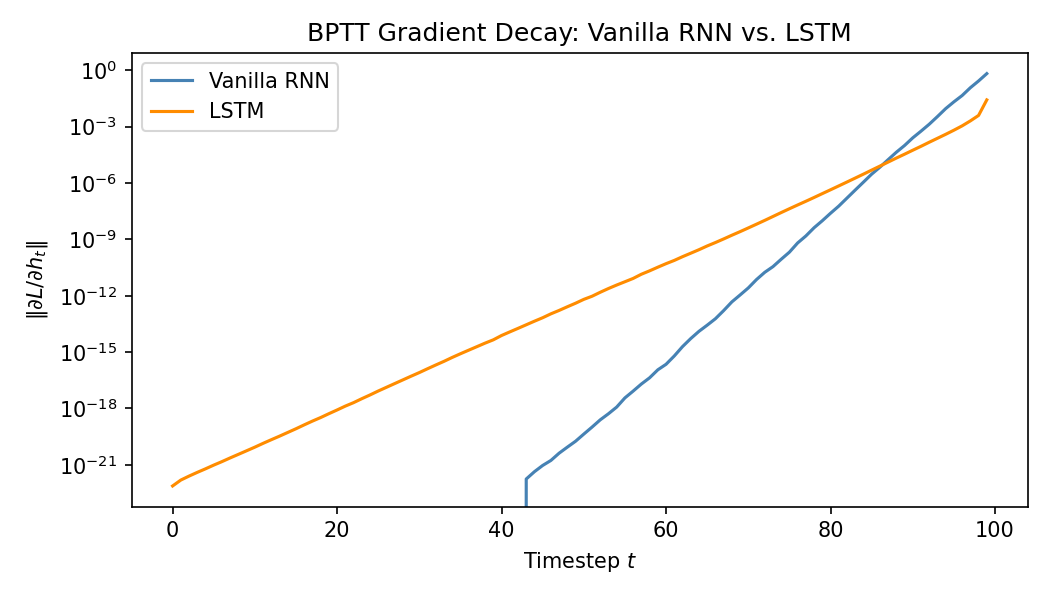
\includegraphics[width=\textwidth]{bptt_decay_comparison.png}
    \caption{BPTT gradient decay: Vanilla RNN vs.\ LSTM (log scale)}
    \label{fig:3_8}
\end{subfigure}
\hfill
\begin{subfigure}[b]{0.48\textwidth}
    \centering
    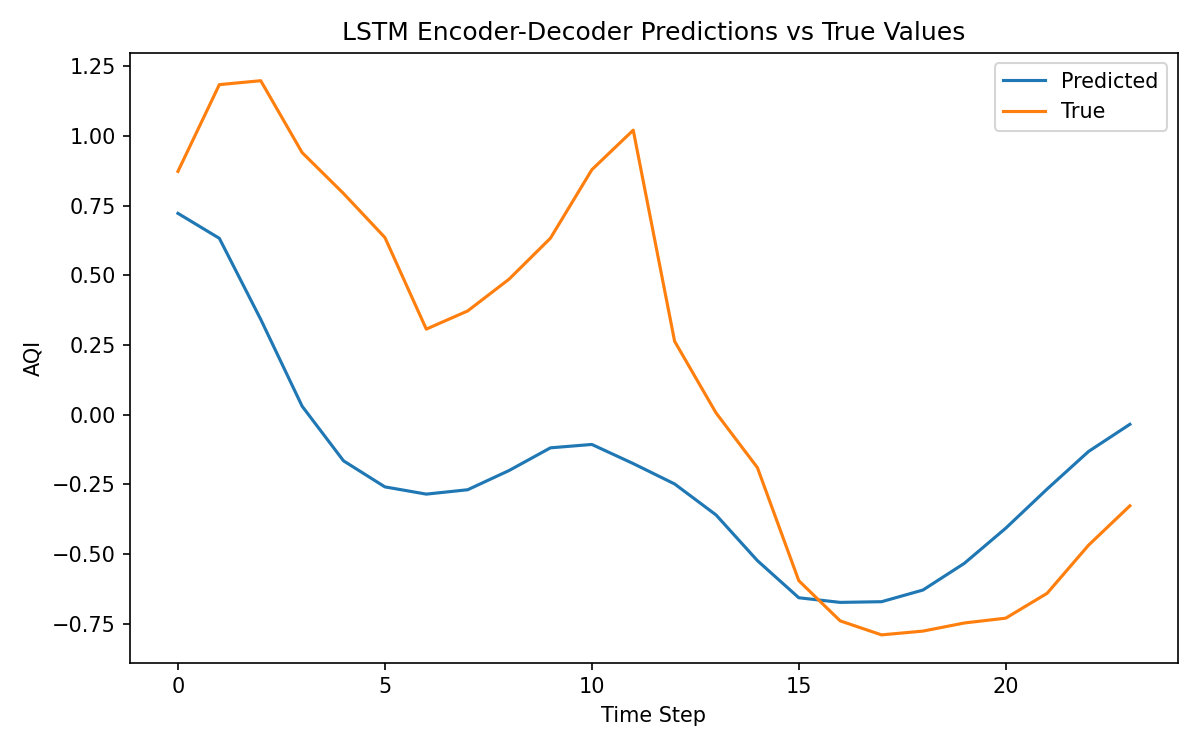
\includegraphics[width=\textwidth]{lstm_encoder_decoder_predictions.png}
    \caption{Encoder-Decoder LSTM: ground truth vs.\ 24-step prediction}
    \label{fig:4_12}
\end{subfigure}
\end{figure}

\questionheader{Phase 5: Transformers \& Attention}

\textbf{5.13 Scaled Dot-Product Attention}
\begin{solution}
Test MSE = \textbf{1.1395}. Fig.~\ref{fig:5_13} shows the $72\times72$ attention weight heatmap; without positional encoding the weights collapse to a near-uniform column, indicating the model cannot distinguish temporal position.
\end{solution}

\textbf{5.14 The Necessity of Positional Encoding}
\begin{solution}
Without PE: best val MSE = 0.2344, test MSE = \textbf{1.1496}. With sinusoidal PE: best val MSE = 0.2295, test MSE = \textbf{0.8872}. Self-attention is permutation-invariant — $\text{Attention}(\pi Q, \pi K, \pi V) = \pi\,\text{Attention}(Q,K,V)$ — so any permutation of the input yields the same output. Without PE, the model fundamentally cannot represent temporal order; adding $\text{PE}(t,2i) = \sin(t/10000^{2i/d})$ breaks this symmetry and injects positional information.
\end{solution}

\textbf{5.15 Vision Transformer (ViT)}
\begin{solution}
Each $128\times128$ image is split into $64$ non-overlapping $16\times16$ patches, each flattened to a 768-dim vector, giving a $(64,768)$ sequence. The same single-head Transformer classifies disease across 38 classes. CNN accuracy: \textbf{86.55\%} with 2,122,470 parameters (efficiency $4.1\times10^{-7}$). Attention accuracy: \textbf{42.43\%} with 64,166 parameters (efficiency $6.6\times10^{-6}$). The ViT is $\approx16\times$ more parameter-efficient.
\end{solution}

\begin{figure}[H]
\centering
\begin{subfigure}[b]{0.48\textwidth}
    \centering
    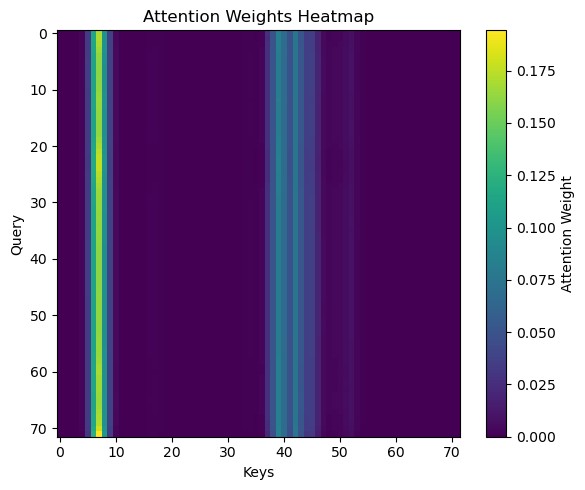
\includegraphics[width=\textwidth]{attention_weights_heatmap.png}
    \caption{$72\times72$ attention weight heatmap (single head, no PE)}
    \label{fig:5_13}
\end{subfigure}
\hfill
\begin{subfigure}[b]{0.48\textwidth}
    \centering
    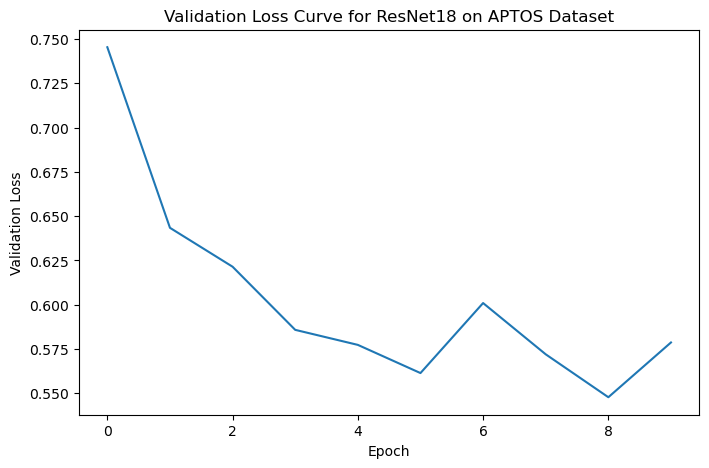
\includegraphics[width=\textwidth]{Validation_loss_resnet_18.png}
    \caption{Validation loss curve: ResNet18 fine-tuning (APTOS 2019)}
    \label{fig:6_16}
\end{subfigure}
\end{figure}

\questionheader{Phase 6: Advanced Vision \& Imbalance (APTOS 2019)}

\textbf{6.16 Transfer Learning \& Freezing}
\begin{solution}
ResNet18 pretrained on ImageNet is loaded; all convolutional layers are frozen. The final FC layer is replaced with \verb|nn.Linear(512, 5)|. Trainable parameters: \textbf{2,565}; total parameters: 11,179,077. Test accuracy: \textbf{77.45\%}, Cohen's Kappa: \textbf{0.6404}. Fig.~\ref{fig:6_16} shows the validation loss curve converging within 10 epochs.
\end{solution}

\textbf{6.17 Ordinal Imbalance \& Focal Loss}
\begin{solution}
The loss is implemented from scratch: $\mathcal{L}_{\text{focal}} = (1-p_t)^\gamma \cdot \mathcal{L}_{\text{CE}}$ with $\gamma=2$, where $p_t = e^{-\mathcal{L}_{\text{CE}}}$. This down-weights well-classified easy examples (large $p_t$) and forces training to focus on hard minority classes. Focal loss test accuracy: \textbf{78.00\%}, Cohen's Kappa: \textbf{0.6496}, vs.\ cross-entropy accuracy: 77.45\%, Kappa: 0.6404 — a consistent improvement on the ordinal metric. Standard cross-entropy accuracy is misleading because Class~0 dominates; a model predicting only Class~0 achieves high accuracy but zero clinical utility. Cohen's QWK penalizes predictions proportionally to their ordinal distance from the true label, making it the appropriate metric for this task.
\end{solution}

\end{document}
